%%%%%%%%%%%%%%%%%%%%%%%%%%%%%%%%%%%%
% Slide options
%%%%%%%%%%%%%%%%%%%%%%%%%%%%%%%%%%%%

% Option 1: Slides with solutions

\documentclass[slidestop,compress,mathserif]{beamer}
\newcommand{\soln}[1]{\textit{#1}}
\newcommand{\solnGr}[1]{#1}

% Option 2: Handouts without solutions

%\documentclass[11pt,containsverbatim,handout]{beamer}
%\usepackage{pgfpages}
%\pgfpagesuselayout{4 on 1}[letterpaper,landscape,border shrink=5mm]
%\newcommand{\soln}[1]{ }
%\newcommand{\solnGr}{ }

%%%%%%%%%%%%%%%%%%%%%%%%%%%%%%%%%%%%
% Style
%%%%%%%%%%%%%%%%%%%%%%%%%%%%%%%%%%%%

\input{../../lec_style.tex}


%%%%%%%%%%%%%%%%%%%%%%%%%%%%%%%%%%%%
% Preamble
%%%%%%%%%%%%%%%%%%%%%%%%%%%%%%%%%%%%

\title[Chp 2: Summarizing data]{Chapter 2: Summarizing data}
\author{OpenIntro Statistics, 4th Edition}
\institute{$\:$ \\ {\footnotesize Slides developed by Mine \c{C}etinkaya-Rundel of OpenIntro. \\
The slides may be copied, edited, and/or shared via the \webLink{http://creativecommons.org/licenses/by-sa/3.0/us/}{CC BY-SA license.} \\
Some images may be included under fair use guidelines (educational purposes).}}
\date{}

%%%%%%%%%%%%%%%%%%%%%%%%%%%%%%%%%%%%
% Begin document
%%%%%%%%%%%%%%%%%%%%%%%%%%%%%%%%%%%%

\begin{document}


%%%%%%%%%%%%%%%%%%%%%%%%%%%%%%%%%%%%
% Title page
%%%%%%%%%%%%%%%%%%%%%%%%%%%%%%%%%%%%

{
\addtocounter{framenumber}{-1} 
{\removepagenumbers 
\usebackgroundtemplate{\includegraphics[width=\paperwidth]{../../OpenIntro_Grid_4_3-01.jpg}}
\begin{frame}

\hfill \includegraphics[width=20mm]{../../oiLogo_highres}

\titlepage

\end{frame}
}
}


%%%%%%%%%%%%%%%%%%%%%%%%%%%%%%%%%%%%
% Sections
%%%%%%%%%%%%%%%%%%%%%%%%%%%%%%%%%%%%

\section{Experiments}

%%%%%%%%%%%%%%%%%%%%%%%%%%%%%%%%%%%%

\begin{frame}
\frametitle{Principles of experimental design}

	\begin{enumerate}
		\item \hl{Control:} Control for the (potential) effect of variables other than the ones directly being studied.
		\item \hl{Randomize:} Randomly assign subjects to treatments, and randomly sample from the population whenever possible.
		\item \hl{Replicate:} Within a study, replicate by collecting a sufficiently large sample. Or replicate the entire study.
		\item \hl{Block:} If there are variables that are known or suspected to affect the response variable, first group subjects into \hl{blocks} based on these variables, and then randomize cases within each block to treatment groups.
	\end{enumerate}

\end{frame}

%%%%%%%%%%%%%%%%%%%%%%%%%%%%%%%%%%%%

\begin{frame}
	\frametitle{More on blocking}

	\twocol{0.25}{0.75}
	{
	\begin{center}
	%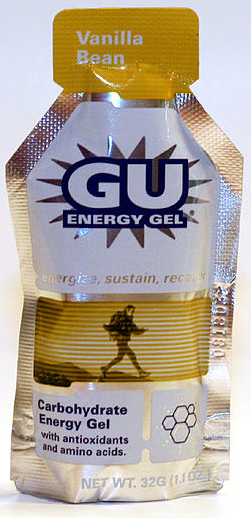
\includegraphics[width=\textwidth]{../../Chp 1/1-4_experiments/figures/gu}
	\end{center}
	}
	{
	\begin{itemize}
		\item We would like to design an experiment to investigate if energy gels make you run faster:
		\pause
		\begin{itemize}
			\item Treatment: energy gel
			\item Control: no energy gel
		\end{itemize}
		\pause
		\item It is suspected that energy gels might affect pro and amateur athletes differently, therefore we block for pro status:
		\pause
		\begin{itemize}
			\item Divide the sample to pro and amateur
			\item Randomly assign pro athletes to treatment and control groups
			\item Randomly assign amateur athletes to treatment and control groups
			\item Pro/amateur status is equally represented in the resulting treatment and control groups
		\end{itemize}
	\end{itemize}
	}

	\pause
	\dq{Why is this important? Can you think of other variables to block for?}

\end{frame}

%%%%%%%%%%%%%%%%%%%%%%%%%%%%%%%%%%%%

% \begin{frame}
% 	\frametitle{Practice}

% 	\pq{A study is designed to test the effect of light level and noise level on exam performance of students. The researcher also believes that light and noise levels might have different effects on males and females, so wants to make sure both genders are equally represented in each group. Which of the below is correct?}

% 	\begin{enumerate}[(a)]
% 		\item There are 3 explanatory variables (light, noise, gender) and 1 response variable (exam performance)
% 		\solnMult{There are 2 explanatory variables (light and noise), 1 blocking variable (gender), and 1 response variable (exam performance)}
% 		\item There is 1 explanatory variable (gender) and 3 response variables (light, noise, exam performance)
% 		\item There are 2 blocking variables (light and noise), 1 explanatory variable (gender), and 1 response variable (exam performance)
% 	\end{enumerate}

% \end{frame}

%%%%%%%%%%%%%%%%%%%%%%%%%%%%%%%%%%%%

\begin{frame}
	\frametitle{Difference between blocking and explanatory variables}

	\begin{itemize}
		\item Factors are conditions we can impose on the experimental units.
		\item Blocking variables are characteristics that the experimental units come with, that we would like to control for.
		\item Blocking is like stratifying, except used in experimental settings when randomly assigning, as opposed to when sampling.
	\end{itemize}

\end{frame}

%%%%%%%%%%%%%%%%%%%%%%%%%%%%%%%%%%%%

\begin{frame}
	\frametitle{More experimental design terminology...}

	\begin{itemize}
		\item \hl{Placebo:} fake treatment, often used as the control group for medical studies
		\item \hl{Placebo effect:} experimental units showing improvement simply because they believe they are receiving a special treatment
		\item \hl{Blinding:} when experimental units do not know whether they are in the control or treatment group
		\item \hl{Double-blind:} when both the experimental units and the researchers who interact with the patients do not know who is in the control and who is in the treatment group

	\end{itemize}

\end{frame}

%%%%%%%%%%%%%%%%%%%%%%%%%%%%%%%%%%%%

% \begin{frame}
% 	\frametitle{Practice}

% 	\pq{What is the main difference between observational studies and experiments?}

% 	\begin{enumerate}[(a)]
% 		\item Experiments take place in a lab while observational studies do not need to.
% 		\item In an observational study we only look at what happened in the past.
% 		\solnMult{Most experiments use random assignment while observational studies do not.}
% 		\item Observational studies are completely useless since no causal inference can be made based on their findings.
% 	\end{enumerate}

% \end{frame}

%%%%%%%%%%%%%%%%%%%%%%%%%%%%%%%%%%%%

\begin{frame}
	\frametitle{Random assignment vs. random sampling}

	\begin{center}
	%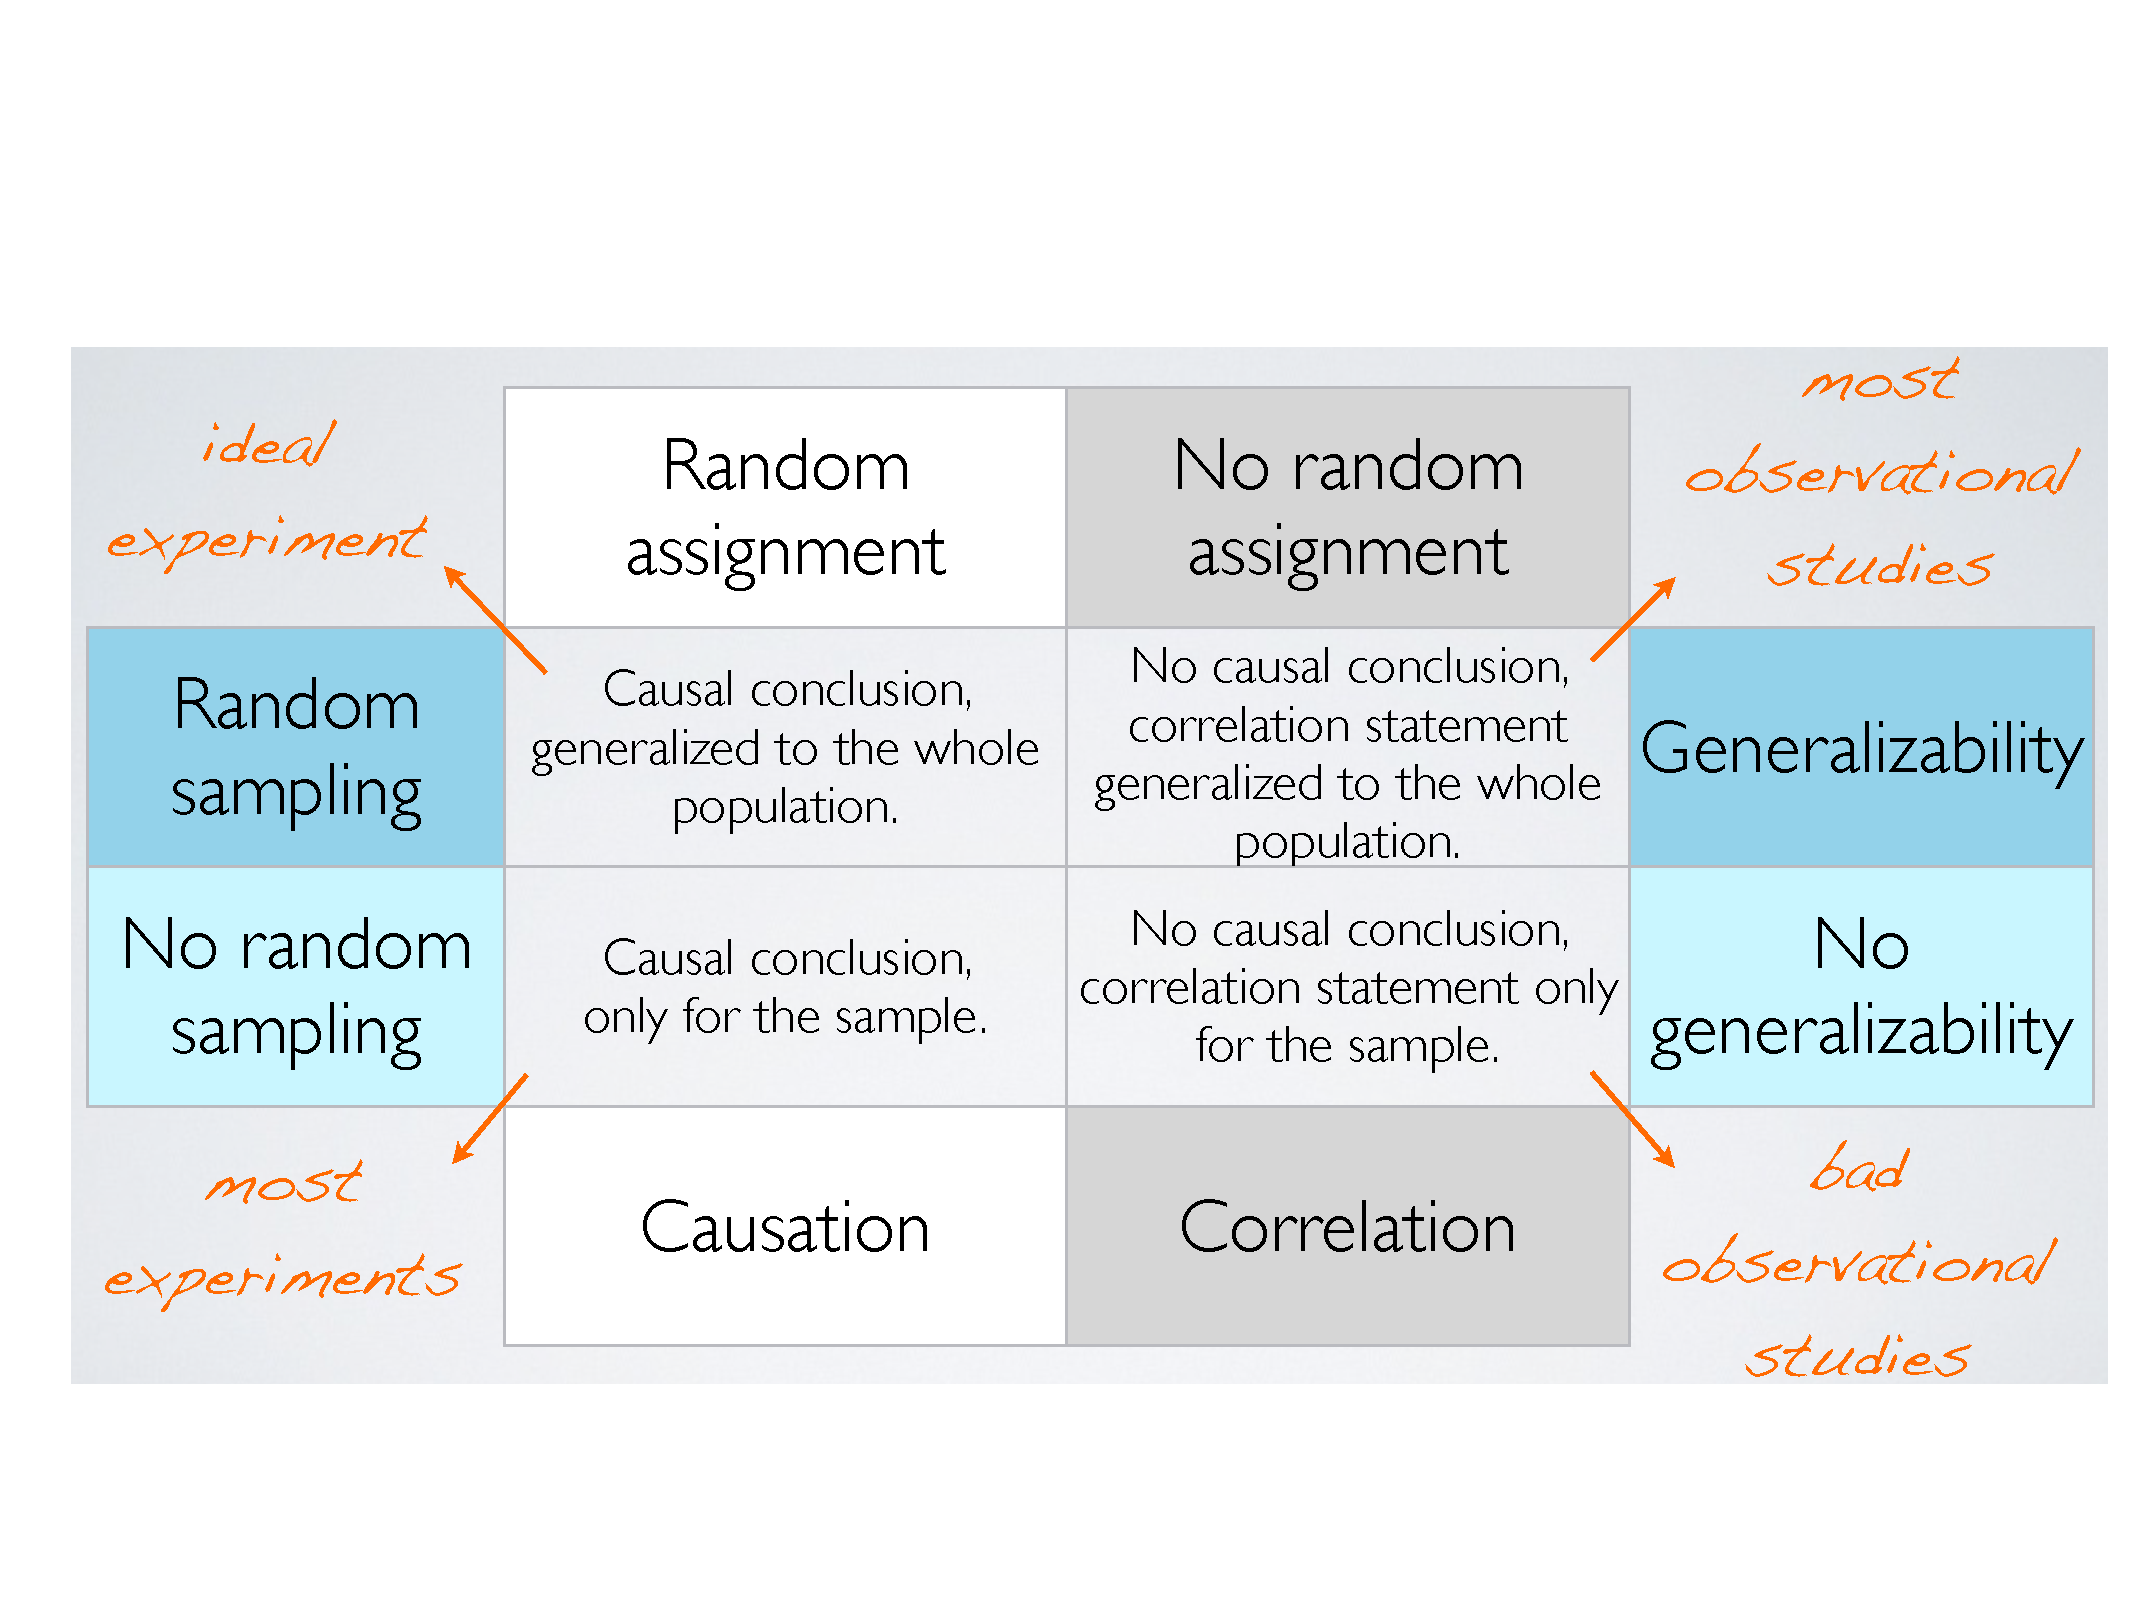
\includegraphics[width=\textwidth]{../../Chp 1/1-4_experiments/figures/random_sample_assignment}
	\end{center}

\end{frame}

%%%%%%%%%%%%%%%%%%%%%%%%%%%%%%%%%%%%

\section{Edfinity Quiz}

%%%%%%%%%%%%%%%%%%%%%%%%%%%%%%%%%%%%

%%%%%%%%%%%%%%%%%%%%%%%%%%%%%%%%%%%%

\section{Examining numerical data}

%%%%%%%%%%%%%%%%%%%%%%%%%%%%%%%%%%%%

\subsection{Scatterplots for paired data}

%%%%%%%%%%%%%%%%%%%%%%%%%%%%%%%%%%%%

\begin{frame}
\frametitle{Scatterplot}

\hl{Scatterplots} are useful for visualizing the relationship between two numerical variables.

\begin{columns}[c]

\column{0.6 \textwidth}

\dq{Do life expectancy and total fertility appear to be \hl{associated} or \hl{independent}?}

\soln{\onslide<2->{They appear to be linearly and negatively associated: as fertility increases, life expectancy decreases.}}

\dq{Was the relationship the same throughout the years, or did it change?}

\soln{\onslide<3->{The relationship changed over the years.}}

\column{0.4 \textwidth}

%%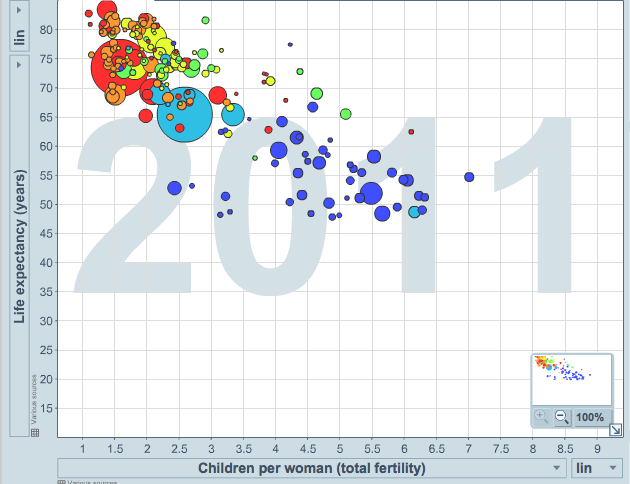
\includegraphics[width=\textwidth]{2-1_numerical_data/figures/life_exp_child}

\end{columns}

\ct{\webURL{http://www.gapminder.org/world}}

\end{frame}

%%%%%%%%%%%%%%%%%%%%%%%%%%%%%%%%%%%%

\subsection{Dot plots and the mean}

%%%%%%%%%%%%%%%%%%%%%%%%%%%%%%%%%%%%

\begin{frame}
\frametitle{Dot plots}

Useful for visualizing one numerical variable. Darker colors represent areas where there are more observations.

\begin{center}
%%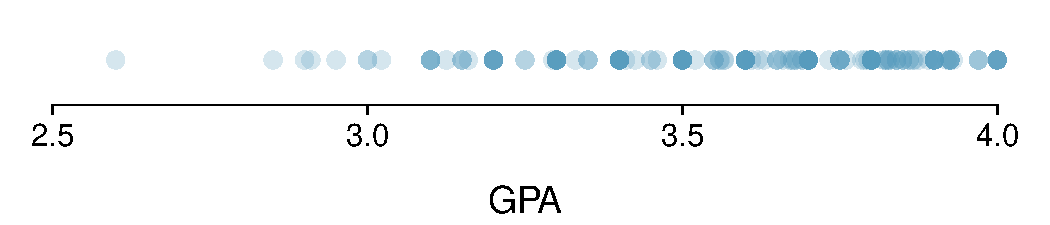
\includegraphics[width=\textwidth]{2-1_numerical_data/figures/gpa_dot_plot/gpa_dot_plot}
\end{center}

\dq{How would you describe the distribution of GPAs in this data set? Make sure to say something about the center, shape, and spread of the distribution.}

\end{frame}

%%%%%%%%%%%%%%%%%%%%%%%%%%%%%%%%%%%%


\begin{frame}
\frametitle{Dot plots \& mean}

\begin{center}
%%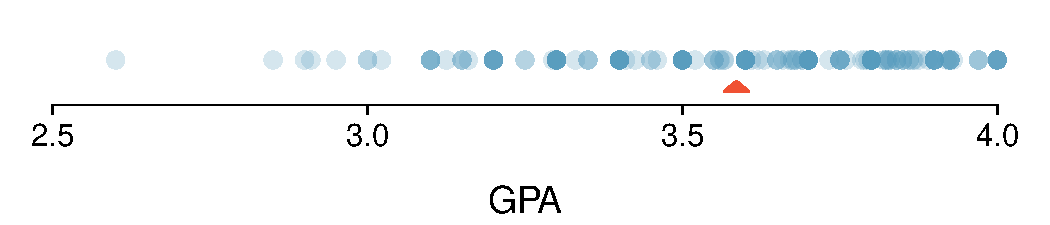
\includegraphics[width=\textwidth]{2-1_numerical_data/figures/gpa_dot_plot/gpa_dot_plot_mean}
\end{center}

\begin{itemize}

\item The \hl{mean}, also called the \hl{average} (marked with a triangle in the above plot), is one way to measure the center of a \hl{distribution} of data.

\item The mean GPA is 3.59.

\end{itemize} 

\end{frame}

%%%%%%%%%%%%%%%%%%%%%%%%%%%%%%%%%%%%

\begin{frame}
\frametitle{Mean}

\begin{itemize}

\item The \hl{sample mean}, denoted as \mathhl{\bar{x}}, can be calculated as

\[ \bar{x} = \frac{x_1 + x_2 + \cdots + x_n}{n}, \]

where $x_1, x_2, \cdots, x_n$ represent the \hl{n} observed values.

\item The \hl{population mean} is also computed the same way but is denoted as \mathhl{\mu}. It is often not possible to calculate $\mu$ since population data are rarely available.

\item The sample mean is a \hl{sample statistic}, and serves as a \hl{point estimate} of the population mean. This estimate may not be perfect, but if the sample is good (representative of the population), it is usually a pretty good estimate. 

\end{itemize}

\end{frame}

%%%%%%%%%%%%%%%%%%%%%%%%%%%%%%%%%%%%

\begin{frame}
\frametitle{Stacked dot plot}

Higher bars represent areas where there are more observations, makes it a little easier to judge the center and the shape of the distribution.

\begin{center}
%%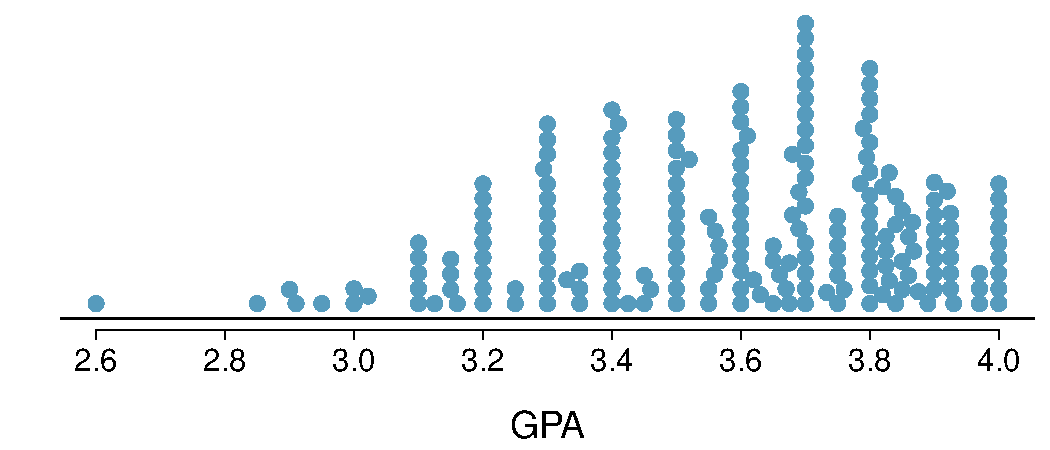
\includegraphics[width=\textwidth]{2-1_numerical_data/figures/gpa_dot_plot/gpa_dot_plot_stacked}
\end{center}

\end{frame}

%%%%%%%%%%%%%%%%%%%%%%%%%%%%%%%%%%%%

\subsection{Histograms and shape}

%%%%%%%%%%%%%%%%%%%%%%%%%%%%%%%%%%%%

\begin{frame}[fragile]
\frametitle{Histograms - Extracurricular hours}

\begin{itemize}

\item Histograms provide a view of the \hl{data density}. Higher bars represent where the data are relatively more common.

\item Histograms are especially convenient for describing the \hl{shape} of the data distribution.

\item The chosen \hl{bin width} can alter the story the histogram is telling.

\end{itemize}

\begin{center}
%%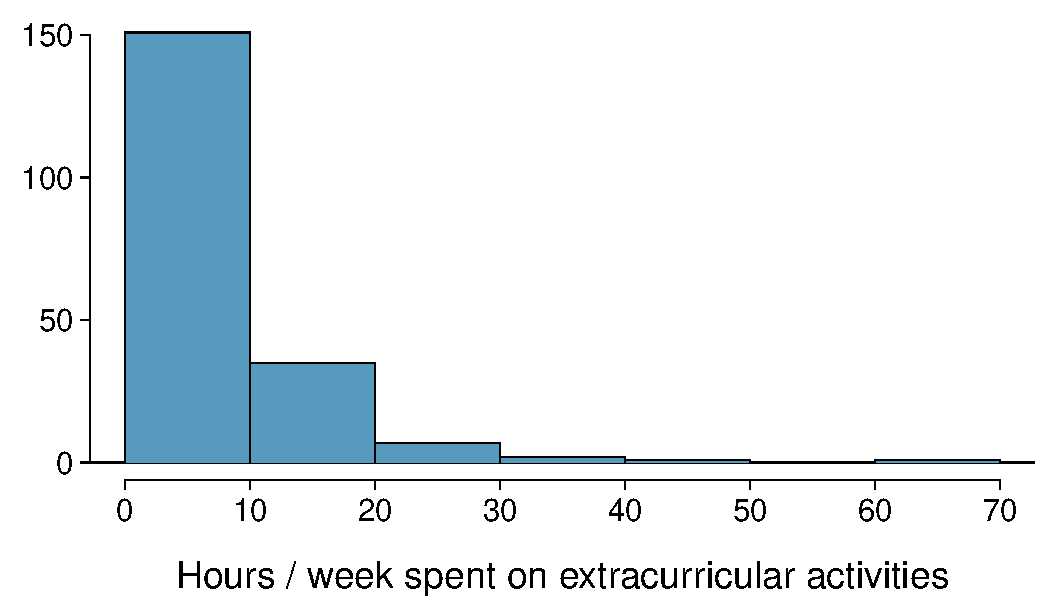
\includegraphics[width=0.75\textwidth]{2-1_numerical_data/figures/extracurr_hrs_hist/extracurr_hrs_hist}
\end{center}

\end{frame}

%%%%%%%%%%%%%%%%%%%%%%%%%%%%%%%%%%%%

\begin{frame}
\frametitle{Bin width}

\dq{Which one(s) of these histograms are useful? Which reveal too much about the data? Which hide too much?}

\begin{center}
%%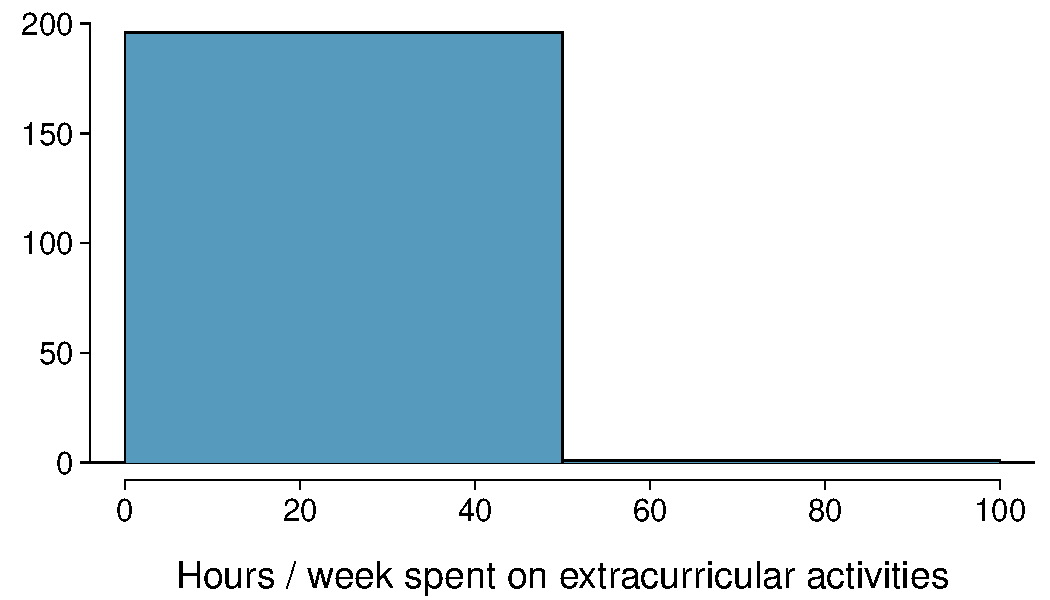
\includegraphics[width=0.45\textwidth]{2-1_numerical_data/figures/extracurr_hrs_hist/extracurr_hrs_hist2}
%%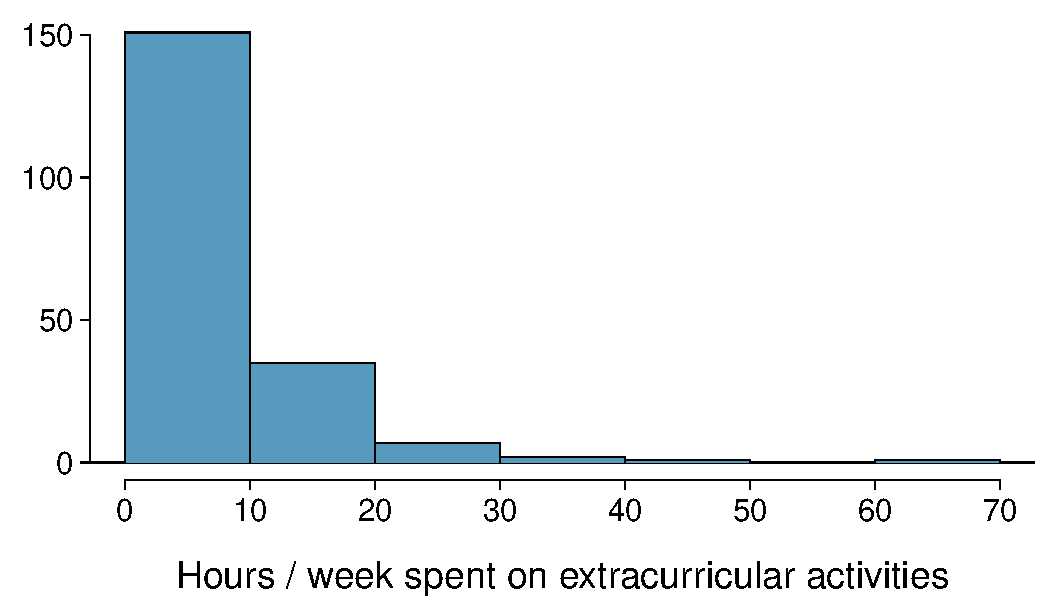
\includegraphics[width=0.45\textwidth]{2-1_numerical_data/figures/extracurr_hrs_hist/extracurr_hrs_hist} \\
%%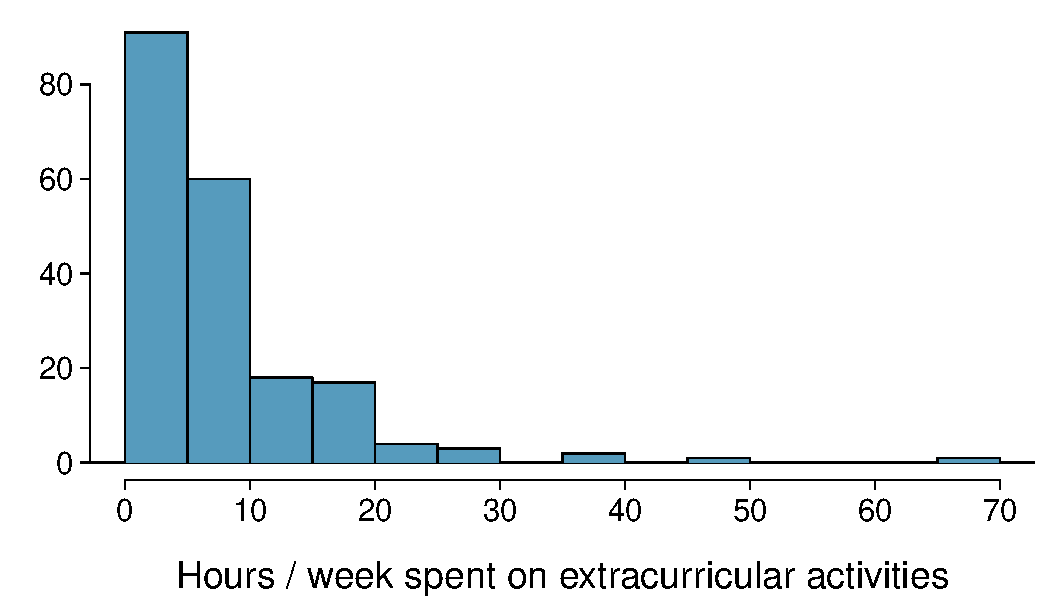
\includegraphics[width=0.45\textwidth]{2-1_numerical_data/figures/extracurr_hrs_hist/extracurr_hrs_hist20}
%%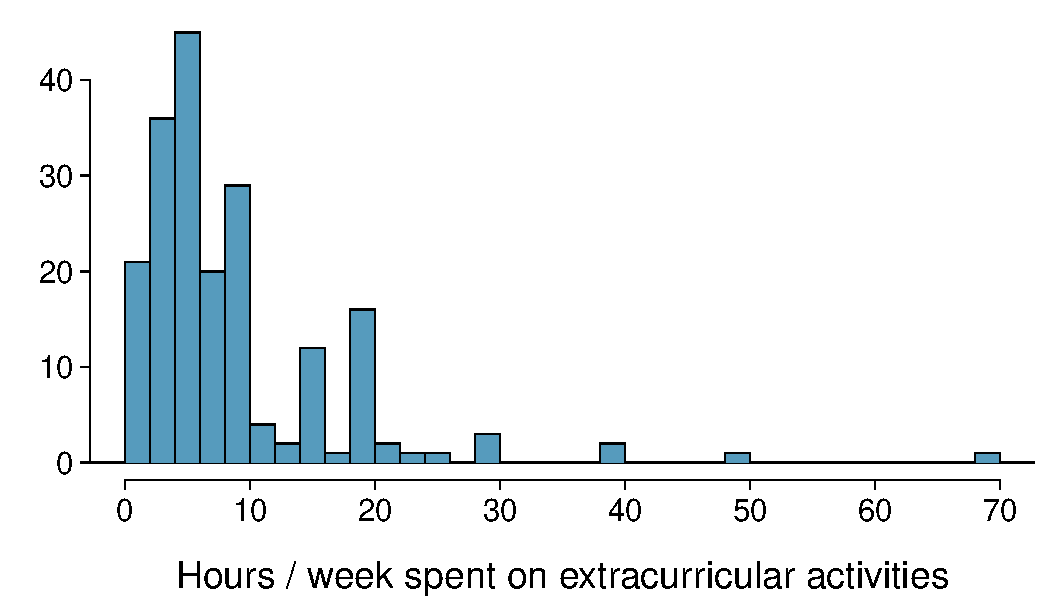
\includegraphics[width=0.45\textwidth]{2-1_numerical_data/figures/extracurr_hrs_hist/extracurr_hrs_hist30}
\end{center}

\end{frame}

%%%%%%%%%%%%%%%%%%%%%%%%%%%%%%%%%%%%

\begin{frame}
\frametitle{Shape of a distribution: modality}

Does the histogram have a single prominent peak (\hl{unimodal}), several prominent peaks (\hl{bimodal/multimodal}), or no apparent peaks (\hl{uniform})?

\begin{center}
%%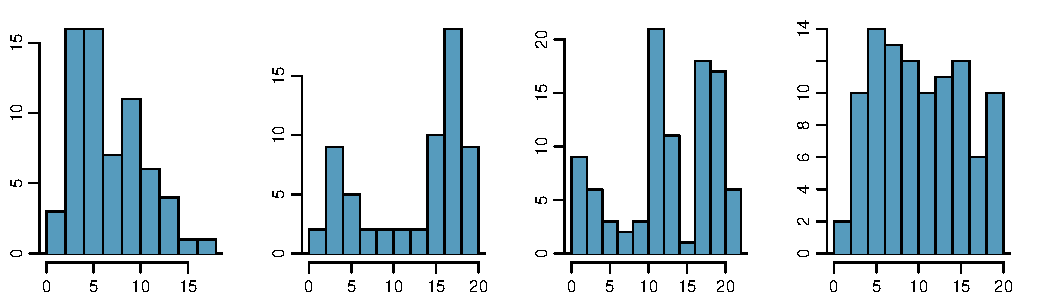
\includegraphics[width=0.75\textwidth]{2-1_numerical_data/figures/singleBiMultiModalUnifPlots/singleBiMultiModalUnifPlots}
\end{center}

\Note{In order to determine modality, step back and imagine a smooth curve over the histogram -- imagine that the bars are wooden blocks and you drop a limp spaghetti over them, the shape the spaghetti would take could be viewed as a smooth curve.}

\end{frame}

%%%%%%%%%%%%%%%%%%%%%%%%%%%%%%%%%%%%

\begin{frame}
\frametitle{Shape of a distribution: skewness}

Is the histogram \hl{right skewed}, \hl{left skewed}, or \hl{symmetric}?

\begin{center}
%%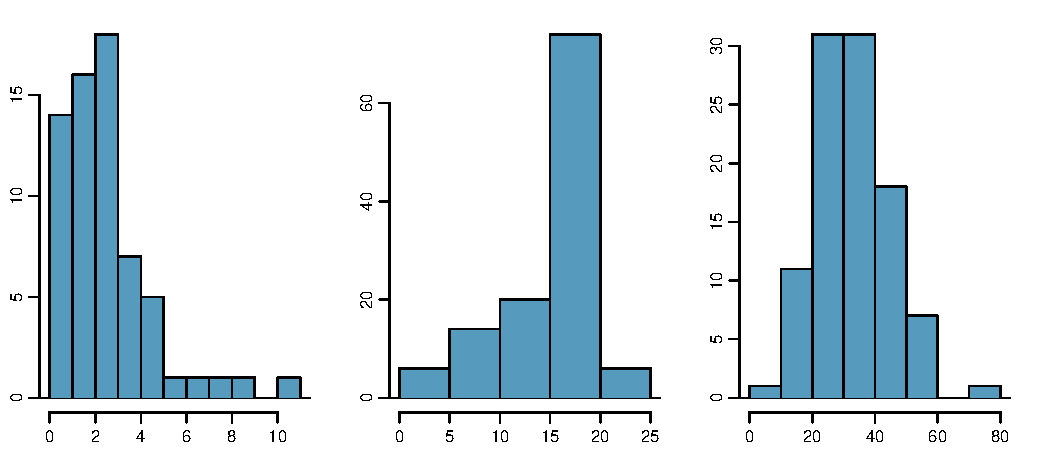
\includegraphics[width=0.8\textwidth]{2-1_numerical_data/figures/skewedSymPlots/skewedSymPlots}
\end{center}

\Note{Histograms are said to be skewed to the side of the long tail.}

\end{frame}

%%%%%%%%%%%%%%%%%%%%%%%%%%%%%%%%%%%%

\begin{frame}
\frametitle{Shape of a distribution: unusual observations}

Are there any unusual observations or potential \hl{outliers}?

\begin{center}
%%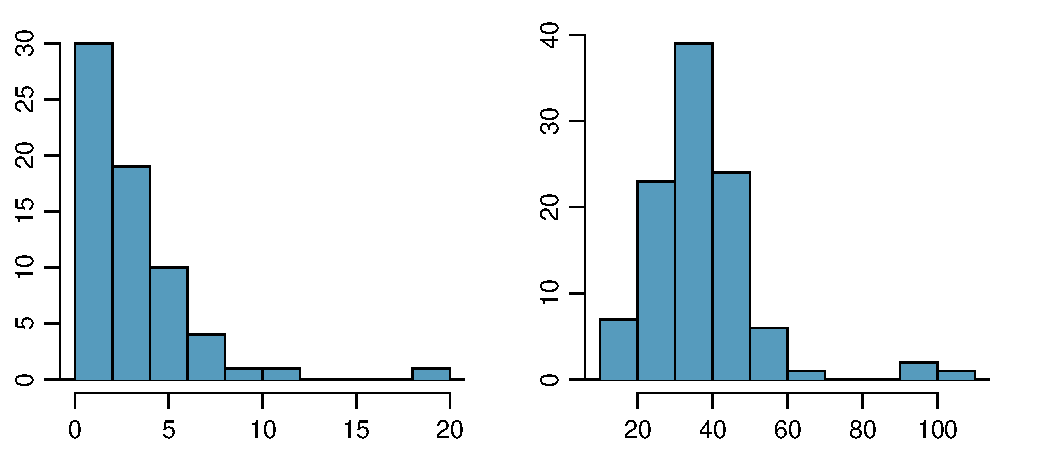
\includegraphics[width=0.8\textwidth]{2-1_numerical_data/figures/outlierPlots/outlierPlots}
\end{center}

\end{frame}

%%%%%%%%%%%%%%%%%%%%%%%%%%%%%%%%%%%%

%\begin{frame}
%\frametitle{Extracurricular activities}

%\dq{How would you describe the shape of the distribution of hours per week students spend on extracurricular activities?}

%\begin{center}
%%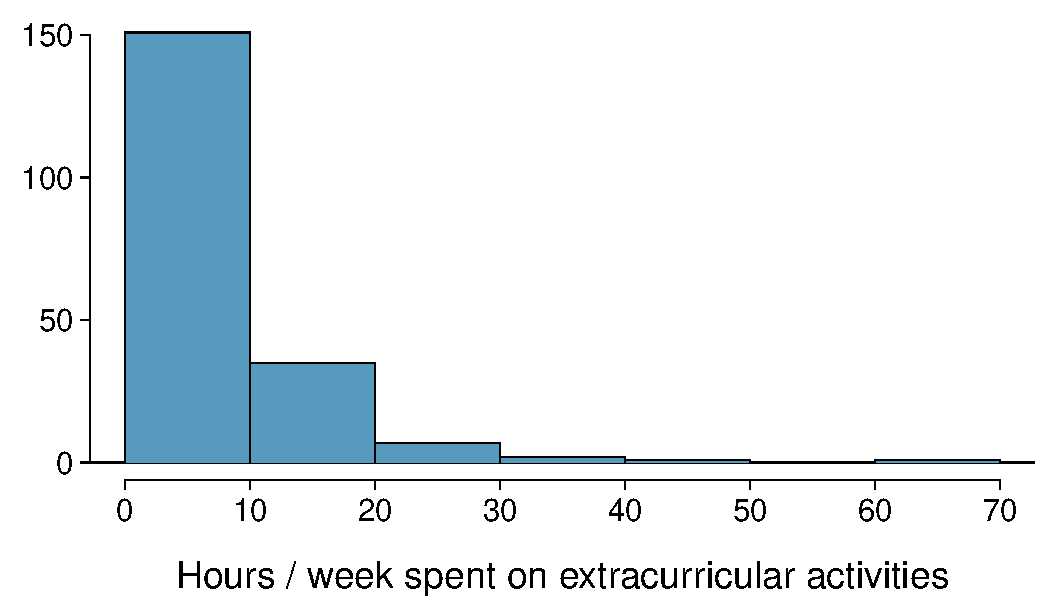
\includegraphics[width=0.75\textwidth]{2-1_numerical_data/figures/extracurr_hrs_hist/extracurr_hrs_hist}
%\end{center}

%\soln{\pause{Unimodal and right skewed, with a potentially unusual observation at 60 hours/week.}}

%\end{frame}

%%%%%%%%%%%%%%%%%%%%%%%%%%%%%%%%%%%%

\begin{frame}
\frametitle{Commonly observed shapes of distributions}

\begin{itemize}

\item modality \\
$\:$ \\
\pause

\begin{columns}[c]
\column{0.25\textwidth}
unimodal \\
%%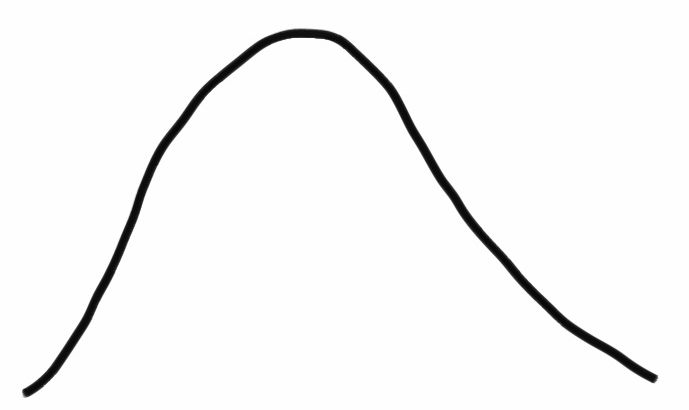
\includegraphics[width=\textwidth]{2-1_numerical_data/figures/shape_sketches/unimodal} 
\pause
\column{0.25\textwidth}
bimodal \\
%%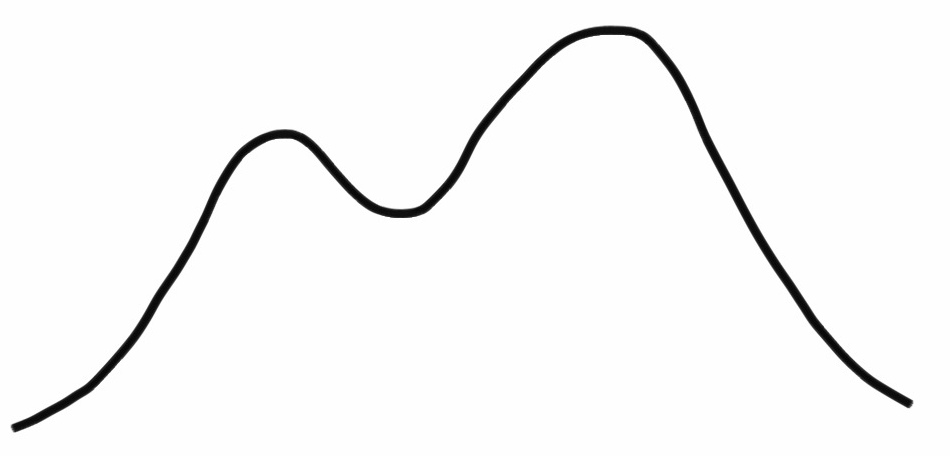
\includegraphics[width=\textwidth]{2-1_numerical_data/figures/shape_sketches/bimodal} 
\pause
\column{0.25\textwidth}
multimodal \\
%%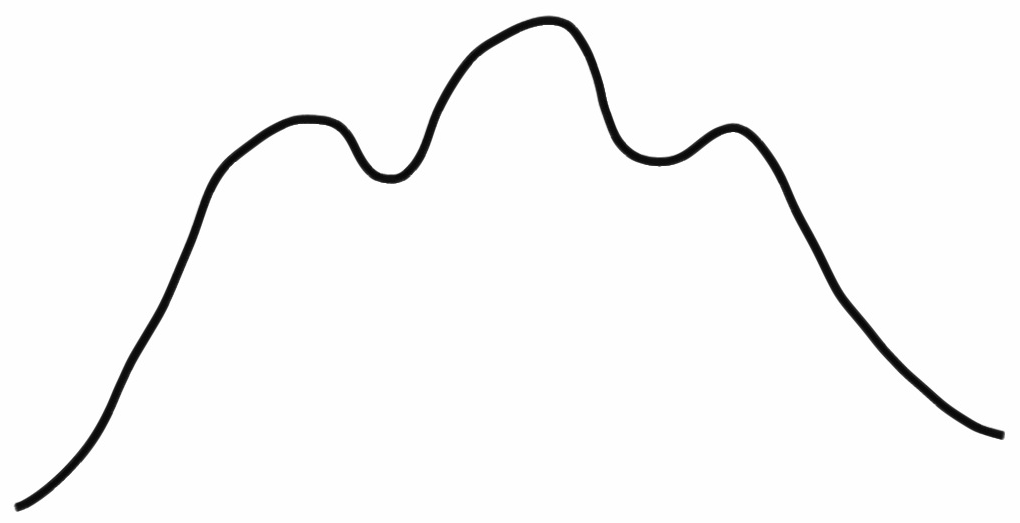
\includegraphics[width=\textwidth]{2-1_numerical_data/figures/shape_sketches/multimodal} 
\pause
\column{0.25\textwidth}
uniform
%%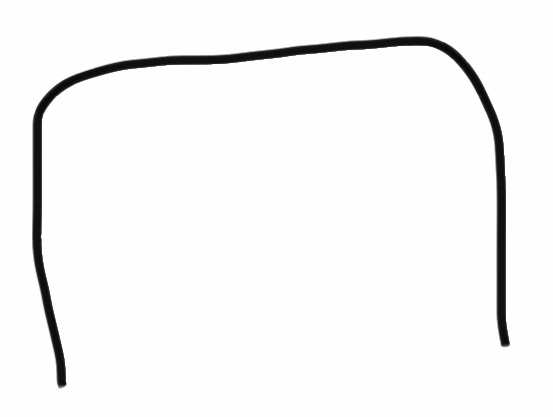
\includegraphics[width=\textwidth]{2-1_numerical_data/figures/shape_sketches/uniform} 
\end{columns}

\pause

$\:$ \\

\item skewness \\
$\:$ \\
\pause

\begin{columns}[c]
\column{0.25\textwidth}
right skew \\
%%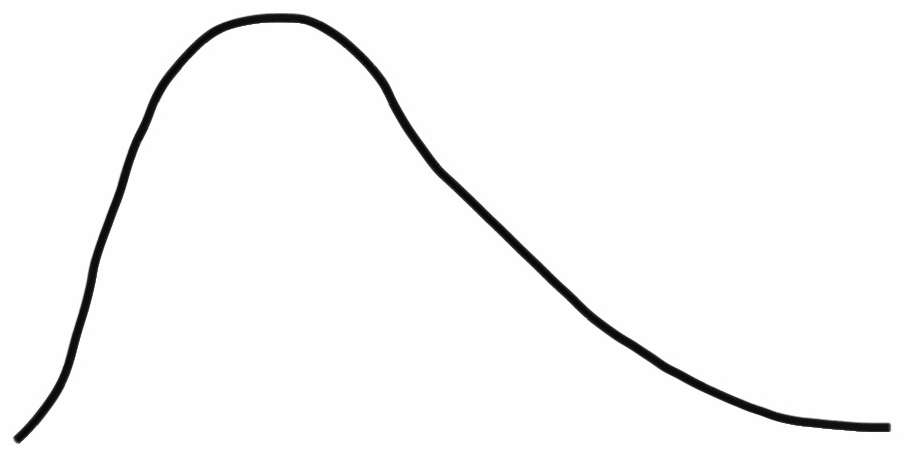
\includegraphics[width=\textwidth]{2-1_numerical_data/figures/shape_sketches/right_skew} 
\pause
\column{0.25\textwidth}
left skew \\
%%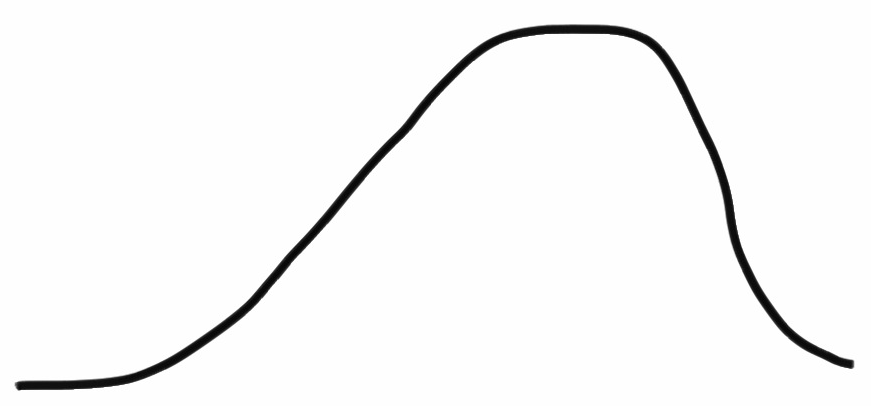
\includegraphics[width=\textwidth]{2-1_numerical_data/figures/shape_sketches/left_skew} 
\pause
\column{0.25\textwidth}
symmetric \\
%%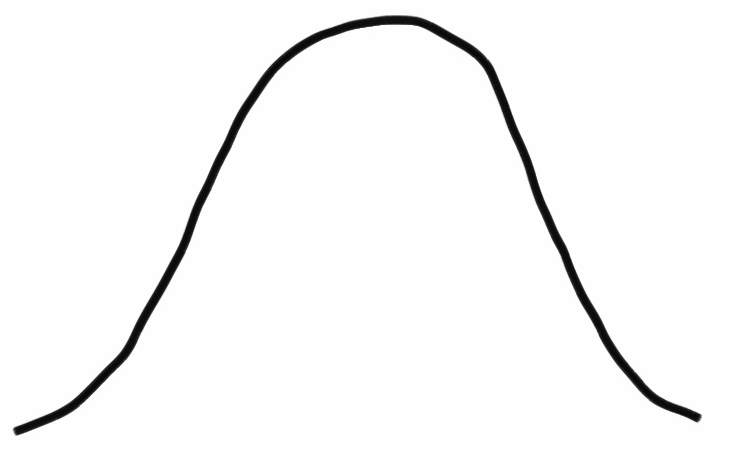
\includegraphics[width=\textwidth]{2-1_numerical_data/figures/shape_sketches/symmetric} 
\end{columns}

\end{itemize}

\end{frame}

%%%%%%%%%%%%%%%%%%%%%%%%%%%%%%%%%%%%

\begin{frame}
\frametitle{Median}

\begin{itemize}

\item The \hl{median} is the value that splits the data in half when ordered in ascending order.

\[ 0,1,\orange{2},3,4 \]

\item If there are an even number of observations, then the median is the average of the two values in the middle.

\[ 0,1,\underline{2,3},4,5 \rightarrow \frac{2 + 3}{2} = \orange{2.5} \]

\item Since the median is the midpoint of the data, 50\% of the values are below it. Hence, it is also the \hl{$50^{th}$ percentile}.

\end{itemize}

\end{frame}



%%%%%%%%%%%%%%%%%%%%%%%%%%%%%%%%%%%
\section{R Demo: Plotting numerical data and computing means}
%%%%%%%%%%%%%%%%%%%%%%%%%%%%%%%%%%%

%%%%%%%%%%%%%%%%%%%%%%%%%%%%%%%%%%%
\section{Edfinity Quiz}
%%%%%%%%%%%%%%%%%%%%%%%%%%%%%%%%%%%

%\begin{frame}
%\frametitle{Practice}

%\pq{Which of these variables do you expect to be uniformly distributed?}

%\begin{enumerate}[(a)]
%\item weights of adult females
%\item salaries of a random sample of people from North Carolina
%\item house prices
%\solnMult{birthdays of classmates (day of the month)}
%\end{enumerate}

%\end{frame}

%%%%%%%%%%%%%%%%%%%%%%%%%%%%%%%%%%%

% TODO: could replicate this activity with an applet in Edfinity
%\begin{frame}
%\frametitle{Application activity: Shapes of distributions}

%\app{Sketch the expected distributions of the following variables:
%\begin{itemize}
%\item number of piercings
%\item scores on an exam
%\item IQ scores
%\end{itemize}
%Come up with a concise way (1-2 sentences) to teach someone how to determine the expected distribution of any variable.
%}

%\end{frame}

%%%%%%%%%%%%%%%%%%%%%%%%%%%%%%%%%%%

\begin{frame}
\frametitle{Are you typical?}

\begin{center}
%%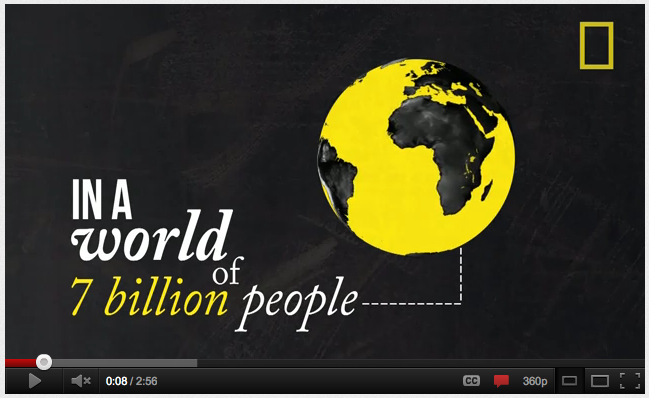
\includegraphics[width=0.75\textwidth]{2-1_numerical_data/figures/typical}
\end{center}

\begin{center}
\footnotesize{\webURL{http://www.youtube.com/watch?v=4B2xOvKFFz4}}
\end{center}

\pause

\dq{How useful are centers alone for conveying the true characteristics of a distribution?}

\end{frame}

%%%%%%%%%%%%%%%%%%%%%%%%%%%%%%%%%%%%

\subsection{Variance and standard deviation}

%%%%%%%%%%%%%%%%%%%%%%%%%%%%%%%%%%%

\begin{frame}
\frametitle{Variance}

\hl{Variance} is roughly the average squared deviation from the mean.

\formula{
\[ s^2 = \frac{\sum_{i = 1}^n (x_i - \bar{x})^2}{n - 1} \]
}

\pause

\twocol{0.5}{0.5}
{
\begin{itemize}

\item The sample mean is $\bar{x} = 6.71$, and the sample size is $n = 217$.

\onslide<3->{\item The variance of amount of sleep students get per night can be calculated as:}
\end{itemize}
}
{
\onslide<2->{
\begin{center}
%%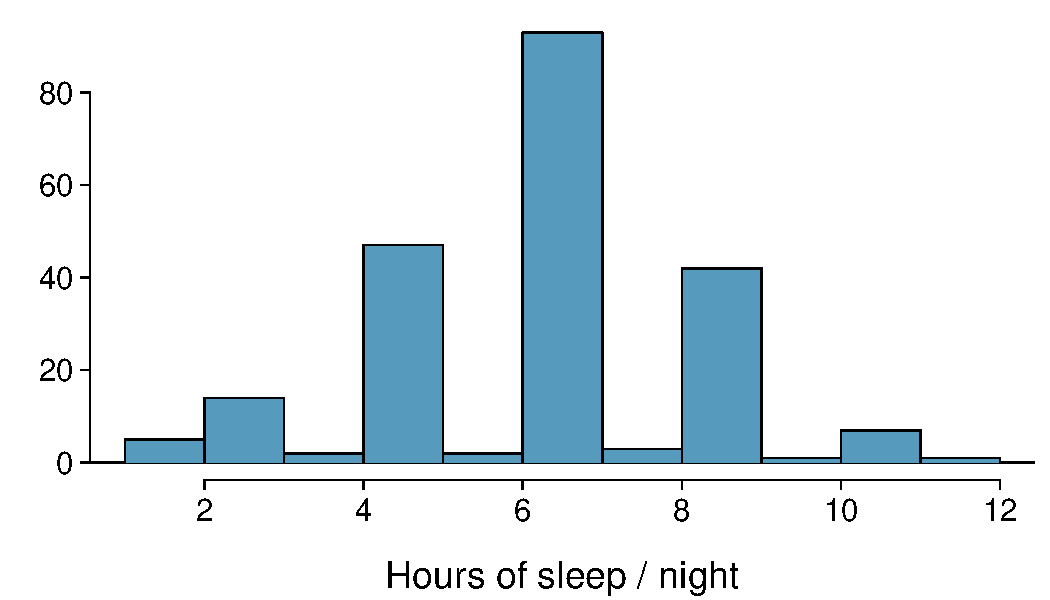
\includegraphics[width=\textwidth]{2-1_numerical_data/figures/sleep_hist/sleep_hist}
\end{center}
}
}
$\:$
\onslide<3->{
\[ s^2 = \frac{(5 - 6.71)^2 + (9 - 6.71)^2 + \cdots + (7 - 6.71)^2}{217 - 1} = 4.11~hours^2 \]
}



\end{frame}

%%%%%%%%%%%%%%%%%%%%%%%%%%%%%%%%%%%

\begin{frame}
\frametitle{Variance (cont.)}

\dq{Why do we use the squared deviation in the calculation of variance?}

\soln{\pause
\begin{itemize}
\item To get rid of negatives so that observations equally distant from the mean are weighed equally.
\item To weigh larger deviations more heavily.
\end{itemize}
}

\end{frame}

%%%%%%%%%%%%%%%%%%%%%%%%%%%%%%%%%%

\begin{frame}
\frametitle{Standard deviation}

The \hl{standard deviation} is the square root of the variance, and has the same units as the data

\formula{
\[ s = \sqrt{s^2} \]
}

\pause

\twocol{0.5}{0.5}
{
\begin{itemize}

\item The standard deviation of amount of sleep students get per night can be calculated as:
\[ s = \sqrt{4.11} = 2.03~hours\]

\onslide<3->{\item We can see that all of the data are within 3 standard deviations of the mean.}
\end{itemize}
}
{
\onslide<2->{
\begin{center}
%%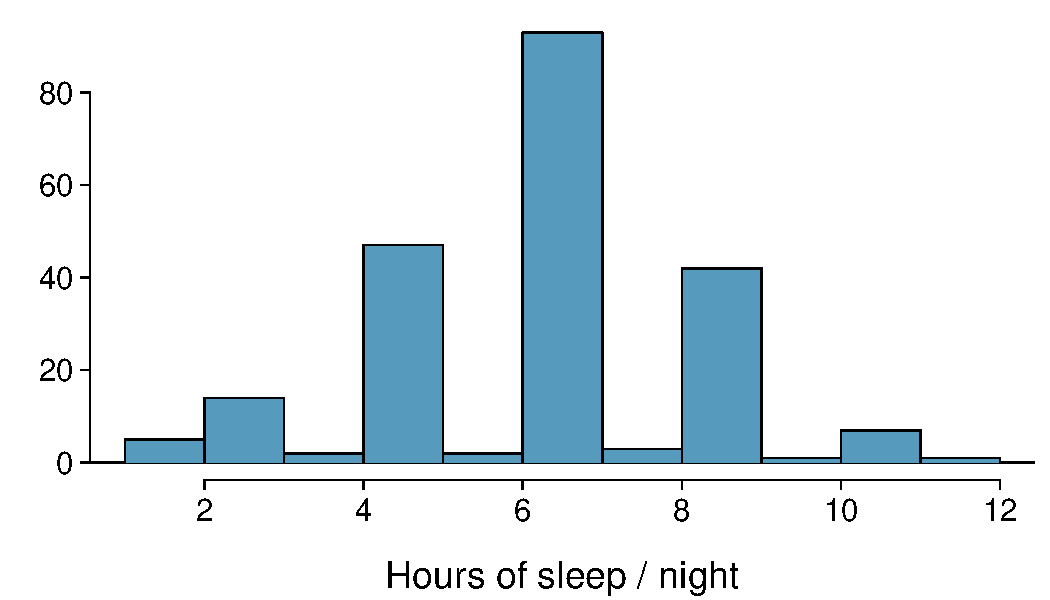
\includegraphics[width=\textwidth]{2-1_numerical_data/figures/sleep_hist/sleep_hist}
\end{center}
}
}

\end{frame}

%%%%%%%%%%%%%%%%%%%%%%%%%%%%%%%%%%%%

\subsection{Box plots and quartiles}

%%%%%%%%%%%%%%%%%%%%%%%%%%%%%%%%%%%%

\begin{frame}[fragile]
\frametitle{Q1, Q3, and IQR}

\begin{itemize}

\item The $25^{th}$ percentile is also called the first quartile, \hl{Q1}.

\item The $50^{th}$ percentile is also called the median.

\item The $75^{th}$ percentile is also called the third quartile, \hl{Q3}.

\item Between Q1 and Q3 is the middle 50\% of the data. The range these data span is called the \hl{interquartile range}, or the \hl{IQR}.
\formula{\[ IQR = Q3 - Q1 \]}
\end{itemize}

\end{frame}

%%%%%%%%%%%%%%%%%%%%%%%%%%%%%%%%%%%
\section{R Demo: Measures of Variability (Variance, StDev, IQR)}
%%%%%%%%%%%%%%%%%%%%%%%%%%%%%%%%%%%

%%%%%%%%%%%%%%%%%%%%%%%%%%%%%%%%%%%%


%%%%%%%%%%%%%%%%%%%%%%%%%%%%%%%%%%%%
% End document
%%%%%%%%%%%%%%%%%%%%%%%%%%%%%%%%%%%%

\end{document}